\documentclass[aspectratio=169]{beamer}

\mode<presentation> {
\usetheme{Goettingen}
\setbeamertemplate{footline}
}

\usepackage{graphicx}
\usepackage{booktabs}
\usepackage{sidecap}
\usepackage{caption}

\title[End of the World scenarios]{Ends of the World are coming}

\author{}
\date{}

\begin{document}

{
\setbeamertemplate{navigation symbols}{}
\usebackgroundtemplate{%
\vbox to \paperheight{\vfil\hbox to \paperwidth{\hfil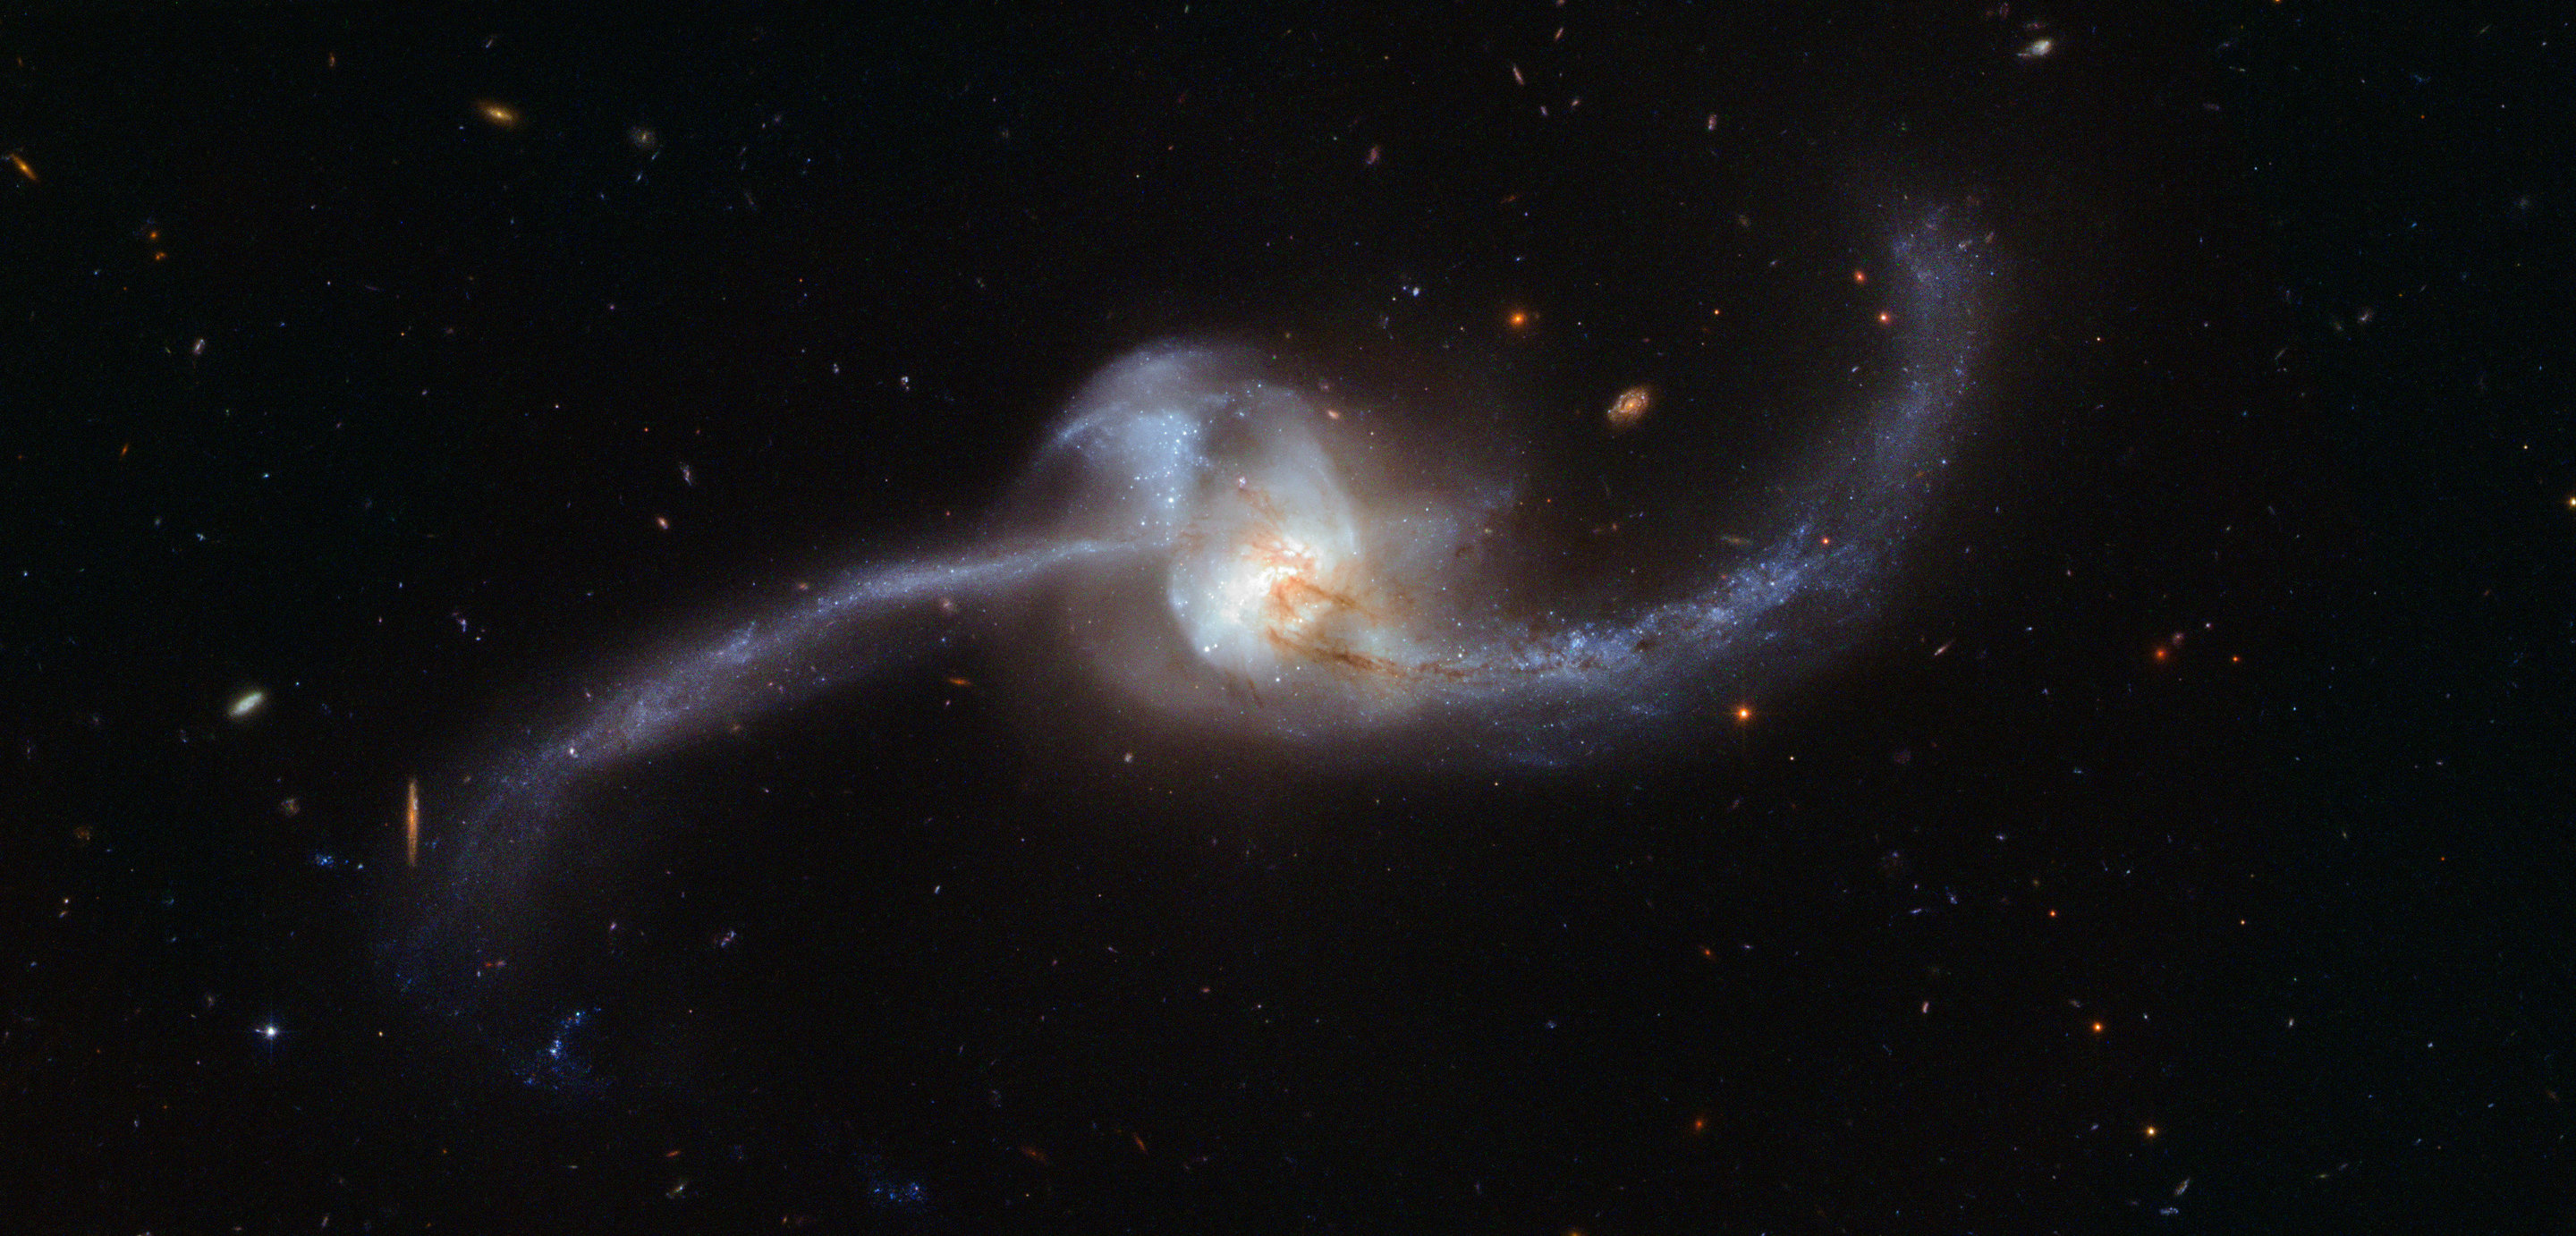
\includegraphics[width=\paperwidth]{img/NGC2623.jpg}\hfil}\vfil}
}
\begin{frame}[plain]
\vspace{-5cm}
\Huge{\centerline{Ends of the World are coming}}
\end{frame}
}

\begin{frame}
\frametitle{Overview}
\tableofcontents
\end{frame}

\section{Definition and classification}

\begin{frame}
\frametitle{What is exactly the End of the World?}
Any natural phenomenon which
\begin{itemize}
\item Causes a mass extinction
      \begin{itemize}
        \item Asteroid impacts
        \item Supernovae explosions
        \item Gamma ray bursts
      \end{itemize}
\item Makes Earth permanently inhospitable to life
      \begin{itemize}
      \item End of the habitable zone
      \end{itemize}
\item Physically destroys Earth
      \begin{itemize}
      \item Red giant stage of the stellar evolution
      \end{itemize}
\end{itemize}
\end{frame}

\section{Asteroid impacts}

\begin{frame}
\frametitle{City killers}
\begin{itemize}
\item An object with $D < 10 \mathrm{m}$ vaporizes in the atmosphere
\item Rocks with a diameter 20 -- 100 m hit the surface.
\end{itemize}

\begin{block}{Is it really that bad?}
\begin{itemize}
\item $\rho \sim 3000 \: \mathrm{kg/m^3}$ (granite)
\item $v \sim 30 - 80 \: \mathrm{km/sec}$ (typical speed of Solar system objects)
\end{itemize}
$E = \frac{m v^2}{2} = \frac{2}{3} \pi \rho R^3 v^2 \sim 10 \: \mathrm{MT}$,
where $1 \: \mathrm{MT} = 4.18 \cdot 10^{15} \mathrm{J}$.
\end{block}
\begin{block}{This happens roughly once a century}
\begin{itemize}
\item 2013 Chelyabinsk meteor 
\item 1908 Tunguska event
\end{itemize}
\end{block}
\end{frame}

\begin{frame}
\frametitle{Massive killing capacity}

\begin{block}{Diameter $\sim 500 \: \mathrm{m}$ (once in $\sim 50000$ years)}
\begin{itemize}
\item Similar to detonating the global nuclear arsenal at once
\item Enough devastate a whole continent
\end{itemize}
\end{block}

\begin{block}{Diameter 2 -- 3 km (once a couple of million years)}
\begin{itemize}
\item Ejects and disperses lots of material
\item It stays in the atmosphere for years and causes a global cooling
\end{itemize}
\end{block}

\begin{block}{Diameter 5 -- 10 km (roughly once in 100 million years)}
\begin{itemize}
\item Nuclear winter lasts decades, oceans get acidified
\item Presumably caused the Cretaceous-Paleogene extinction (poor dinosaurs)
\end{itemize}
\end{block}
\end{frame}

\section{Supernova explosions}

\begin{frame}
\frametitle{Supernova explosions}
\begin{columns}[c]
\column{0.55\textwidth}
\begin{figure}
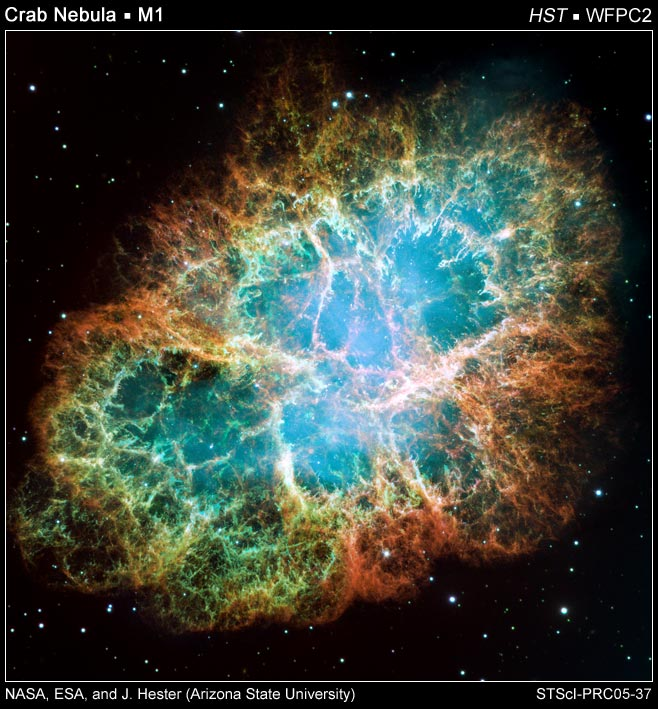
\includegraphics[width=0.95\textwidth]{img/crab_nebula_web_print.jpg}
\end{figure}
\column{0.45\textwidth}
\begin{itemize}
\item Heavy stars ($M > 8 M_\odot$) collapse at the end of the lifetime
\item Collapse causes a huge thermonuclear explosion
\item During a few weeks supernova outshines a whole galaxy
\item Supernovae occur once a 50 years in a galaxy of Milky Way size
\end{itemize}
\end{columns}
\end{frame}

\begin{frame}
\frametitle{Supernova explosions}
\begin{itemize}
\item Explosion sprays EM radiation and ultra-relativistic particles
\item Life on a planet closer than 50 -- 100 LY is in a trouble
\item There are no dangerous stars at such distances for now
\item In the future the Sun might move to a less cozy place
\end{itemize}
\end{frame}

\section{Gamma ray bursts}
\begin{frame}
\frametitle{Gamma ray bursts}
\begin{block}{Supernova explosions of rapidly rotating stars}
\begin{itemize}
\item Powerful magnetic fields form during the collapse
\item Magnetic fields focus the explosion products
\item Narrow streams might be deadly even at $\sim 10000$~LY
\end{itemize}
\end{block}
\begin{block}{Other causes}
\begin{itemize}
\item Neutron stars mergers
\item Black holes mergers
\end{itemize}
\end{block}
\end{frame}

\begin{frame}
\frametitle{GRB safety notice}

\begin{block}{Do I need to run to a radiation shelter?}
\begin{enumerate}
\item It's too late (most GRB are seconds to minutes long)
\item Most of GRB radiation gets blocked by the atmosphere
\end{enumerate}
\end{block}

\begin{block}{Any dangerous stars around?}
Perhaps \href{https://en.wikipedia.org/wiki/WR_104}{WR 104} in 8000 LY
\end{block}

\begin{block}{How often GRBs happen close enough to Earth?}
A rough estimate: once in 1 Gyr
\end{block}
\end{frame}

\begin{frame}
\frametitle{Why exactly GRBs are harmful?}
\begin{block}{Global cooling}
\begin{itemize}
\item Gamma rays break $N_2$ and $O_2$ molecules into atoms
\item Which recombine into nitrogen oxides $NO$, $NO_2$
\item These molecules can float in the stratosphere for years
\item $NO_2$ efficiently blocks the visible light
\end{itemize}
\end{block}

\begin{block}{Mass extinction due to increased UV level}
\begin{itemize}
\item $NO$ destroys ozone: $NO + O_3 \to NO_2 + O_2$
\item Solar UV level at the Earth surface increases
\item 30\% solar UV increase is enough to kill phytoplankton 
\end{itemize}
\href{http://en.wikipedia.org/wiki/Ordovician\%E2\%80\%93Silurian_extinction_events}{Ordovician-Silurian mass extinction}
(44O Myr ago) might have been caused by an GRB \cite{arXiv:astro-ph/0309415}
\end{block}
\end{frame}


\section{End of the habitable zone}
\begin{frame}
\frametitle{Sun evolution at the main sequence}
\begin{figure}
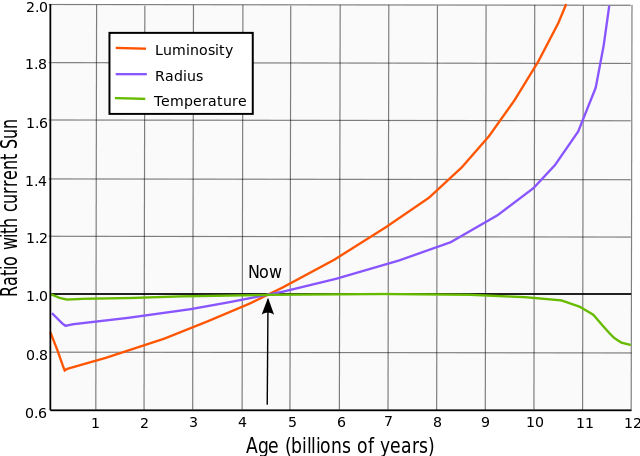
\includegraphics[width=0.7\textwidth]{img/640px-Solar_evolution_(English).png}
\captionsetup{labelformat=empty}
\caption{Evolution of the Solar luminosity, radius, and temperature \cite{arXiv:0911.4872}}
\end{figure}
\end{frame}

\begin{frame}
\frametitle{Consequences for life on Earth}

\begin{itemize}
\item{Photosynthesis shutdown in 800 Myr}
\item{Loss of oceans in 1 Gyr}
\item{Extinction of the remaining life forms in 2.8 Gyr}
\end{itemize}
\end{frame}


\begin{frame}{Photosynthesis shutdown}
Rocks slowly convert atmospheric $CO_2$ into carbonate minerals:
\begin{displaymath}
\nonumber
Ca Si O_3 + CO_2 + H_2 O \to 2 H CO_3^- + Ca^{2+} + Si O_2
\end{displaymath}

\begin{itemize}
\item The rate rapidly increases with the temperature
\item In 600 Myr $CO_2$ concentration will be 50 PPM \cite{arXiv:0912.2482} versus the current 400 PPM
\item 50 PPM is too low for \href{http://en.wikipedia.org/wiki/C3_carbon_fixation}{$C_3$ carbon fixation}
\item Vast majority of plants use $C_3$ process, these will die (including all trees)
\item Plants relying on \href{http://en.wikipedia.org/wiki/C4_carbon_fixation}{$C_4$ carbon fixation} will follow in 200~Myr
\end{itemize}
\end{frame}


\begin{frame}
\frametitle{Loss of oceans}
\begin{itemize}
\item A 10\% increase of the solar luminosity bumps the global surface temperature to 32O K ($47^\circ \mathrm{C}$)
\item The atmosphere will become a "moist greenhouse" leading to runaway
  evaporation of oceans \cite{James F. Kasting}
\item The stratosphere will contain increasing levels of water
\item Solar ultraviolet will break water molecules into oxygen and hydrogen
\item Light hydrogen molecules easily escape to the space
\item Net result: loss of all ocean water in 1 Gyr
\end{itemize}

Note: oceans don't need to boil for this to happen
\end{frame}

\begin{frame}
\frametitle{Extinction of the remaining life forms}
\begin{itemize}
\item There will be several oceans worth of water in the mantle \cite{Bounama}
\item Lots of microbes will definitely move and adapt
\item In 2.8 Gyr from now: $T_{surface} = 422 \: \mathrm{K}$ ($149^\circ \mathrm{C}$)
\item All life forms will be extinguished due to extreme conditions
\item Remaining water might cause further runaway moist greenhouse effect
\item The surface temperature will raise to 1600 K (enough to melt the surface)
\end{itemize}
\end{frame}

\section{Milky Way and Andromeda merger}
\begin{frame}
\frametitle{Milky Way and Andromeda}
\only<1>{
\begin{figure}
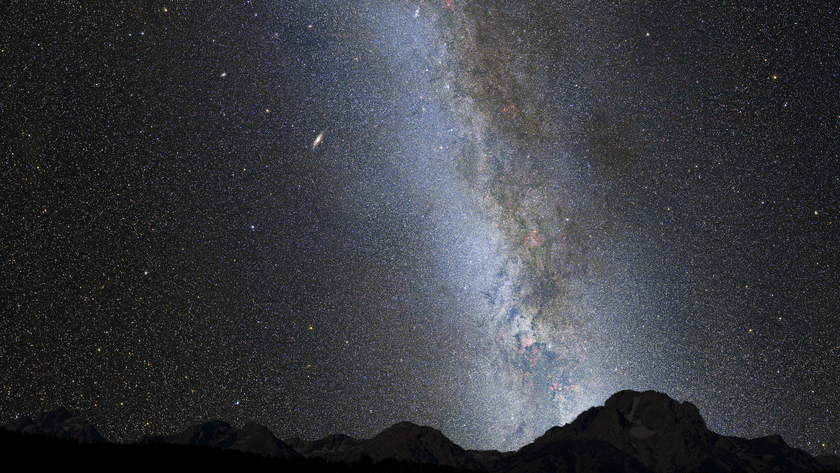
\includegraphics[width=\textwidth]{img/20120929_andromeda_collision_1-present_hs-2012-20-c_f840.png}
\captionsetup{labelformat=empty}
\caption{now}
\end{figure}
}
\only<2>{
\begin{figure}
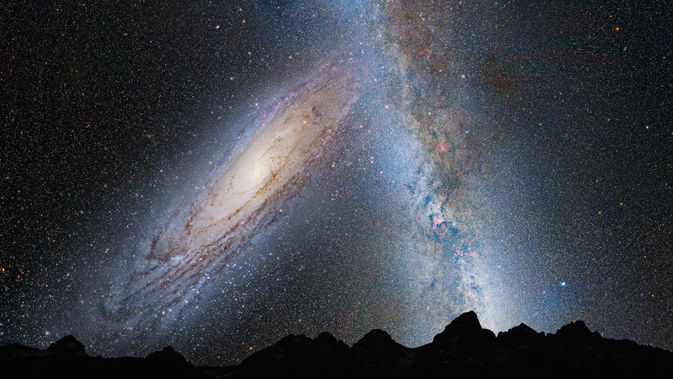
\includegraphics[width=\textwidth]{img/milkdromeda.jpg}
\captionsetup{labelformat=empty}
\caption{in $\sim 3.5$ Gyr from now}
\end{figure}
}
\transdissolve<2>
\end{frame}

\begin{frame}
\frametitle{Milky Way and Andromeda merger}
\begin{itemize}
\item Andromeda is approaching us at $\sim 110 \: \mathrm{km/sec}$.
\item That's not enough for collision: the transverse speed matters.
\item According to recent measurements by Hubble space telescope
      \cite{arXiv:1205.6864}
      and Gaia mission \cite{arXiv:1805.04079} Andromeda will
      definitely hit us.
\item ETA: 3.75 -- 4.5 billion years.
\item Stellar collisions are extremely unlikely: $D(\alpha Cen - \odot) \sim 3 \cdot 10^7 D_\odot$ 
\end{itemize}
\end{frame}

\begin{frame}
\frametitle{Super massive black holes merger}
\begin{itemize}
\item A super massive black hole (SMBH) of $3.6 \cdot 10^6 M_\odot$ resides at the center of Milky Way
\item A SMBH of $1 - 2 \cdot 10^8 M_\odot$ resides at the center of Andromeda
\item They will converge near the center of the newly formed galaxy and merge
\item Nearby ordinary stars will be slingshotted to higher radius orbits or ejected from the galaxy
\item Gas clouds attracted by SMBHs could create a quasar ($\sim 10^7$ supernova explosions)
\item Stars passing too close to SMBH can be torn apart by the tidal force
\end{itemize}

\end{frame}

\begin{frame}
\frametitle{Burst of star formation}
\begin{itemize}
\item Gas clouds collide and compress, and form new stars
\item The Sun can acquire heavy neighbors which can go supernova in a couple of million years
\item At that time Earth would be lifeless anyway
\end{itemize}
\end{frame}

\section{Other Ends of the World}
\begin{frame}
\frametitle{Further Ends of the World}
\begin{itemize}
\item Sun goes red giant and expands beyond the current Earth orbit, ETA: 5 Gyr
\item Accelerated expansion of space-time drags all galaxies beyond the cosmological horizon, ETA: 600 Gyr
\item Last (red dwarf) star dies, ETA: 100 Tyr
\item Planetary system dissolved by close encounters between stellar remnants, ETA: $10^{15}$ yr
\item Galaxies dissolution: heavier bodies fall to the center, and lighter fling into the void, ETA: $10^{18}$ yr
\item Last black hole evaporates, ETA: $10^{100}$ yr
\end{itemize}
\end{frame}

\begin{frame}
\Large{\centerline{Quantum fluctuations may spawn new Universes}}
\Large{\centerline{ETA: $10^{10^{10^{\ldots}}}$}}
\end{frame}


\section{References}
\begin{frame}[allowframebreaks]
\footnotesize{

\begin{thebibliography}{99}
\bibitem{arXiv:astro-ph/0309415}%
A. Melott, B. Lieberman, C. Laird, L. Martin, M. Medvedev, B. Thomas (University of Kansas), J. Cannizzo, N. Gehrels, C. Jackman (NASA-Goddard) 
\newblock Did a gamma-ray burst initiate the late Ordovician mass extinction?
\newblock \href{http://arxiv.org/abs/astro-ph/0309415}{astro-ph/0309415}

\bibitem{arXiv:0911.4872}I. Ribas (2009)
\newblock The Sun and stars as the primary energy input in planetary atmospheres
\newblock \href{http://arxiv.org/abs/0911.4872}{arXiv:0911.4872}

\bibitem{arXiv:0912.2482}Martin J. Heath, Laurance R. Doyle
\newblock Circumstellar Habitable Zones to Ecodynamic Domains: A Preliminary Review and Suggested Future Directions
\newblock \href{http://arxiv.org/abs/0912.2482}{arXiv:0912.2482}

\bibitem{Bounama}Bounama, C., Franck, S., and von Bloh, W. (2001)
\newblock The fate of Earth's ocean
\newblock \href{http://doi.org/10.1016/0019-1035(88)90116-9}{Hydrol. Earth Syst. Sci., 5, 569-576}

\bibitem{James F. Kasting}
\newblock Runaway and moist greenhouse atmospheres and the evolution of Earth and Venus
\newblock \href{https://doi.org/10.1016/0019-1035(88)90116-9}{Icarus (ISSN 0019-1035), vol. 74, June 1988, p. 472-494.}

\bibitem{arXiv:1205.6864}Roeland P. van der Marel, Mark Fardal, Gurtina Besla, Rachael L. Beaton, Sangmo Tony Sohn, Jay Anderson, Tom Brown, Puragra Guhathakurta
\newblock The M31 Velocity Vector. II. Radial Orbit Towards the Milky Way and Implied Local Group Mass
\newblock \href{http://arxiv.org/abs/1205.6863}{arXiv:1205.6864}

\bibitem{arXiv:1805.04079}Roeland P. van der Marel, Mark A. Fardal, Sangmo Tony Sohn, Ekta Patel, Gurtina Besla, Andrés del Pino-Molina, Johannes Sahlmann, Laura L. Watkins
\newblock First Gaia Dynamics of the Andromeda System: DR2 Proper Motions, Orbits, and Rotation of M31 and M33
\newblock \href{http://arxiv.org/abs/1805.04079}{arXiv:1805.04079}

\end{thebibliography}
}
\end{frame}

\end{document} 
